% Certifying Safe Operating Regions under Monotone Failure Modes
% Draft for ICML 2027. Uses icml2027.sty / icml2026.sty when present (drop
% the file next to this one); otherwise falls back to a two-column layout
% with ICML-like margins so the draft compiles anywhere.
\documentclass{article}

\usepackage{amsmath,amssymb,amsthm}
\usepackage{booktabs}
\usepackage{graphicx}
\usepackage{xcolor}
\usepackage{natbib}
\usepackage{hyperref}

\newif\ificmlstyle
\IfFileExists{icml2027.sty}{\usepackage{icml2027}\icmlstyletrue}{%
  \IfFileExists{icml2026.sty}{\usepackage{icml2026}\icmlstyletrue}{%
    \usepackage[letterpaper,top=1in,bottom=1in,left=0.75in,right=0.75in,columnsep=0.25in]{geometry}%
    \usepackage{times}}}

\newtheorem{theorem}{Theorem}
\newtheorem{lemma}{Lemma}
\newtheorem{corollary}{Corollary}
\newtheorem{definition}{Definition}
\newtheorem{assumption}{Assumption}
\renewcommand{\theassumption}{A}

\newcommand{\TBD}[1]{\textcolor{red}{[TBD: #1]}}
\newcommand{\eps}{\varepsilon}
\newcommand{\KL}{\mathrm{KL}}
\newcommand{\kl}{\mathrm{kl}}
\newcommand{\cX}{\mathcal{X}}
\newcommand{\preceqm}{\preceq_m}
\newcommand{\Cone}{\mathcal{C}}
\newcommand{\E}{\mathbb{E}}
\renewcommand{\P}{\mathbb{P}}

\begin{document}

\ificmlstyle
\twocolumn[
\icmltitle{Certifying Safe Operating Regions under Monotone Failure Modes}
\begin{icmlauthorlist}\icmlauthor{Anonymous}{anon}\end{icmlauthorlist}
\icmlaffiliation{anon}{Anonymous institution}
\icmlcorrespondingauthor{Anonymous}{anon@example.com}
\vskip 0.3in]
\printAffiliationsAndNotice{}
\else
\twocolumn[{\centering
{\Large\bfseries Certifying Safe Operating Regions under Monotone Failure Modes\par}
\vspace{0.8em}{Anonymous authors\par}\vspace{1.5em}}]
\fi

\begin{abstract}
Many systems are configured by a few continuous knobs, and each setting can
fail in more than one way: a language model sampled at low temperature
degenerates into repetition and at high temperature into incoherence; a
laser powder bed fusion process at low energy leaves unmelted powder and at
high energy drills keyhole pores. Practitioners need the \emph{safe
operating region}, the settings where every failure mode is rare. Each
failure rate can only be estimated from trials at that very setting, so
evaluating a grid of configurations costs in proportion to its area. We
study \emph{certifying a safe region with a family-wise guarantee when every
configuration needs its own trials}, using the one piece of structure these
systems share: each failure mode is monotone in known directions. We give
(i) the \emph{cone rule}, a closed-testing procedure with betting
e-processes that is valid at any stopping time and under any adaptive
choice of trials, and under monotonicity reduces to two cumulative sums;
(ii) a \emph{search algorithm} for the fixed-confidence problem that stops
on its own once the target region is certified; (iii) lower bounds showing
that with the ordering the cost is governed by the region's \emph{edge} and
without it by its \emph{area}, and an upper bound for the search within
logarithmic and multiple-testing factors of the ordered lower bound. On
sampling settings of a language model \TBD{LM numbers}, on additive
manufacturing process windows and on a drug-combination screen, the method
needs 1.3--9$\times$ fewer trials than adaptive testing without the
ordering and, on $48\times48$ grids, 19--26$\times$ fewer than a full grid
with Learn-then-Test fixed-sequence testing, with no unsafe setting
certified in any run,
while a Gaussian-process level-set baseline certifies unsafe settings in
7.5--100\% of runs unless it certifies almost nothing.
\end{abstract}

% =====================================================================
\section{Introduction}

A team deploying a language model must choose sampling settings
(temperature, top-$p$). Too low, and outputs repeat themselves; too high,
and they stop making sense. They want a region of settings where, with
95\% confidence, both failure rates are below 10\%, so that any setting in
it is safe to ship. A setting's failure rates can only be estimated by
generating outputs at that setting and judging them, which is expensive at
scale. The same pattern appears in process qualification for additive
manufacturing (laser power $\times$ scan speed; lack of fusion
vs.\ keyholing), in dose finding for drug combinations (toxicity vs.\ lack
of response), and in operating envelopes of controllers.

\paragraph{What we ask for.} A certified region $C$ such that, with
probability at least $1-\alpha$, every setting in $C$ has every failure
rate below its tolerance. The guarantee must hold when the experimenter looks at results after
every batch and stops whenever they like, and however the next trials are
chosen, including by an imperfect simulator or model.

\paragraph{Why existing tools fall short.}
\emph{Risk control for configurations} (Learn-then-Test
\citep{angelopoulos2025ltt}; Pareto Testing \citep{laufer2023pareto};
Conformal Language Modeling \citep{quach2024conformal}; MultiRisk
\citep{joshi2025multirisk}) evaluates every candidate configuration on a
shared calibration set. When evaluating a configuration means fresh trials
at it, that costs the full grid; we compare against Learn-then-Test's
fixed-sequence testing, which uses monotonicity along one axis, and find it
needs 19--26$\times$ more trials than our method at $48\times 48$.
\emph{Adaptive multiple testing with bandits} \citep{jamieson2018bandit,
xu2021unified} samples adaptively but treats configurations as unrelated.
\emph{Monotone thresholding bandits} \citep{garivier2017dose,
cheshire2020shape} use order in one dimension, for one constraint, without
anytime validity. \emph{Safe Bayesian optimization and GP level-set
estimation} \citep{sui2015safeopt, gotovos2013lse, losalka2023monotone,
losalka2024noregret} rely on the GP model being right; their certificates
fail when it is not (Section~\ref{sec:exp}).

\paragraph{Structure.} In all these systems each failure mode is monotone
in known directions (repetition falls with temperature, incoherence rises
with it). The null hypotheses ``setting $x$ is unsafe for mode $m$'' are
therefore logically related: if $x$ is unsafe, so is everything riskier
than $x$.

\paragraph{Contributions.}
\begin{enumerate}
\item \emph{Problem.} Certification of a safe region under per-mode partial
orders when each configuration needs its own trials, in a fixed-budget and
a fixed-confidence version (Section~\ref{sec:problem}).
\item \emph{Testing.} The cone rule: closed testing with weighted e-values,
which under monotonicity is a cumulative sum; valid at every time under
arbitrary adaptive sampling (Section~\ref{sec:cone}).
\item \emph{Allocation.} For a fixed budget, trials at the riskiest
uncertified settings of a slightly shrunken target (the lower bound's
binding constraints). For fixed confidence, a galloping/bisection search
along the ordering with a two-sided probe that never stalls near a
threshold (Section~\ref{sec:alloc}).
\item \emph{Theory.} Lower bounds with and without the ordering (edge
vs.\ area); upper bounds by Wald's identity; the search is within
$O(\log n)$ and multiple-testing factors of the ordered lower bound
(Section~\ref{sec:theory}).
\item \emph{Experiments.} Sampling settings of a language model, additive
manufacturing (a Rosenthal melt-pool model and a synthetic window), and a
drug-combination screen (Section~\ref{sec:exp}).
\end{enumerate}

% =====================================================================
\section{Problem}\label{sec:problem}

Configurations form a grid $\cX = [n_1]\times[n_2]$, $N = n_1 n_2$. There
are $M$ failure modes. A trial at $x$ yields $Y\in\{0,1\}^M$, i.i.d.\ given
$x$ (modes may be dependent). The failure rate is $p_m(x) = \E Y_m$; $x$ is
\emph{safe} if $p_m(x) < \eps_m$ for all $m$, and the safe region is $W$.

\begin{assumption}[monotone failure modes]
For each $m$ there is a known product order $\preceqm$ on $\cX$ such that
$x \preceqm y$ implies $p_m(y) \le p_m(x)$ (``$y$ is at least as safe as
$x$ for mode $m$'').
\end{assumption}

\paragraph{Protocol.} Trials are requested in batches; each batch is chosen
from all data so far and any side information (a simulator, a cheaper
model, a pilot study) before its outcomes are seen.

\paragraph{Fixed budget.} Output certified sets $C_t$ with
$\P(C_t\subseteq W \ \forall t) \ge 1-\alpha$, and make $C_t$ large.

\paragraph{Fixed confidence.} For a slack $q<1$ and target
$T = \{x : p_m(x)\le q\eps_m\ \forall m\}$, stop at a time $\tau$ with a
certified set $C$.
\begin{definition}
A procedure is \emph{$(\alpha,\beta)$-correct} if for every instance
satisfying Assumption~A: (validity) $\P(C\not\subseteq W)\le\alpha$, and
(completeness) $\P(\tau<\infty,\ T\subseteq C)\ge 1-\beta$.
\end{definition}
Settings with rates between $q\eps$ and $\eps$ may be certified or not.

% =====================================================================
\section{Testing: the cone rule}\label{sec:cone}

\paragraph{Per-configuration evidence.} For each $(m,x)$, a betting
e-process
$K_{m,x}(t) = \prod_{s\le t:\,x_s=x}\bigl(1+\lambda_s(\eps_m - Y_{s,m})\bigr)$,
with $\lambda_s\in[0, c/(1-\eps_m)]$, $c<1$, chosen before trial $s$. Under
$H_{m,x}: p_m(x)\ge\eps_m$ it is a nonnegative supermartingale for the
filtration generated by all trials and side information
(Lemma~\ref{lem:supermart}). We bet with a hedge: half a plug-in bet seeded
by side information \citep{waudbysmith2024betting}, half a mixture of eight
fixed bets.

\paragraph{The rule.} Fix weights $w_{m,x}\ge0$ with $\sum w\le 1$ before
the trials. Let $\Cone_m(x) = \{y : y\preceqm x\}$ be the riskier cone of
$x$ (including $x$). Certify $x$ for mode $m$ once
\begin{equation}\label{eq:cone}
S_m(x,t) = \sum_{y\in\Cone_m(x)} w_{m,y} K_{m,y}(t) \ \ge\ 1/\alpha,
\end{equation}
and certify $x$ once it is certified for every mode. For a product order
on a grid, $S_m$ for all $x$ is two cumulative sums.

\begin{theorem}[validity]\label{thm:valid}
Under Assumption~A, for any allocation and stopping time,
\[
\P\bigl(\exists\, t, (m,x):\ p_m(x)\ge\eps_m,\ x \text{ certified for $m$ by } t\bigr)\le\alpha.
\]
\end{theorem}
\begin{proof}[Proof sketch]
The unsafe pairs $D$ are closed toward risk, so a false certification of
$x$ gives
\[
1/\alpha\le S_m(x,t)\le E(t) := \textstyle\sum_{(m,y)\in D} w_{m,y}K_{m,y}(t),
\]
a nonnegative supermartingale starting at most 1; apply Ville's inequality.
Full proof in Appendix~\ref{app:valid}.
\end{proof}

This is closed testing \citep{marcus1976closed} with the weighted
e-value intersection test \citep{vovk2021evalues}: monotonicity makes the
smallest true intersection containing $(m,x)$ a cone, so the closure is a
cumulative sum. A certificate at $x$ automatically covers every safer
setting, and evidence from riskier settings is pooled.

\paragraph{Weights.} Certifying $x$ with weight $w$ takes about
$\ln(1/(\alpha w))$ divided by $\KL(p\|\eps)$ trials, so weights should sit on
likely edge points. We use the frequency with which a setting is an edge
point of the target under perturbed side information (logit shifts),
mixed 50/50 with uniform weights.

% =====================================================================
\section{Allocation}\label{sec:alloc}

\paragraph{Fixed budget: the edge rule.} Estimate the target with slack
(all estimated rates below $0.7\eps$); for each mode, run trials at the
riskiest uncertified settings of that estimate, several per batch, cheapest
first; then re-check uncertified settings whose lower confidence bound
still admits membership. These are the binding constraints of the lower
bound (Theorem~\ref{thm:lb}a).

\begin{figure}[t]
\fbox{\begin{minipage}{0.95\columnwidth}\small
\textbf{Algorithm 1} (search, fixed confidence)\\[2pt]
\textbf{Input:} grid, modes and orders, $\eps$, $q$, $\alpha$, $\beta$,
side information.\\
\textbf{Probe}$(m,x)$: run trials at $x$ until $S_m(x)\ge1/\alpha$
(certify $x$ and everything safer for $m$) or $R_{m,x}\ge MN/\beta$
(reject $x$ and everything riskier for $m$).\\
\textbf{For} each mode $m$ and row $j$, riskiest rows first:\\
\hspace*{1em}$s\gets$ edge found in an adjacent row, else predicted edge;\\
\hspace*{1em}\textbf{gallop}: probe $s$, then $s\pm1,s\pm2,s\pm4,\dots$
toward the side the outcome points to, until the outcome flips;\\
\hspace*{1em}\textbf{bisect} the undecided positions of the bracket
until every position is certified or rejected.\\
\textbf{Stop} when every (mode, setting) is certified, rejected, or
excluded (rejected for another mode); output the certified settings.
\end{minipage}}
\end{figure}

\paragraph{Fixed confidence: search (Algorithm 1).} For each mode and each row (a chain
of the order), run a \emph{two-sided probe} at one setting at a time:
certify it by the cone rule, or reject ``$p_m(x)\le q\eps_m$'' with a
failure-betting e-process at level $\beta/(MN)$. A certificate spreads to
safer settings, a rejection to riskier ones. Start at the edge found in an
adjacent row (or the side information's predicted edge), gallop until the
edge is bracketed, then bisect. Stop when every row is decided for every
mode. Because $q<1$, at every rate at least one side of the probe has
positive drift, so no probe stalls.

% =====================================================================
\section{Theory}\label{sec:theory}

Let $K_1=\kl(1-\beta,\alpha)$, and for $\pi\in[0,1]$ let
$f(\pi)=\kl(\pi,1-\beta)$ for $\pi<1-\beta$ (else 0) and
$g(\pi)=\kl(\pi,\alpha)$ for $\pi>\alpha$ (else 0). Write
$\KL_m(y)=\KL(p_m(y)\|\eps_m)$ when $p_m(y)<\eps_m$ and 0 otherwise.

\begin{theorem}[lower bound]\label{thm:lb}
Any $(\alpha,\beta)$-correct procedure has $\E[\tau]\ge\mathrm{OPT}$, the
value of the convex program: minimize $\sum_y n_y$ over $n\ge0$ subject to
\begin{itemize}
\item[(i)] for each $m$ and each riskiest point $t$ of $T$ (for $\preceqm$):
$\sum_{y\preceqm t} n_y\KL_m(y)\ge K_1$;
\item[(ii)] for each $m$ and each \emph{boundary point} $z$ ($z\notin T$
only because of mode $m$, and every setting strictly safer than $z$ for $m$
is in $T$ for $m$): $(A_z,B_z)\in R$, where
\[
R=\{(A,B):\ \exists\pi\ \ A\ge f(\pi),\ B\ge g(\pi)\},
\]
$A_z=n_z\KL(p_m(z)\|q\eps_m)$ and $B_z=\sum_{y\preceqm z}n_y\KL_m(y)$.
\end{itemize}
Without the ordering, every setting must be resolved on its own and the
bound is a sum of per-setting terms over all of $\cX$.
\end{theorem}
The binding points of (i) form an antichain (at most $\min(n_1,n_2)$ per
mode), and so do those of (ii): with the ordering the bound involves
at most $2M\min(n_1,n_2)$ settings, without it all $N$.

\begin{theorem}[oracle upper bound]\label{thm:oracle}
Running trials only at a cover of $T$ costs at most
$\sum_{\text{cover}}(\ln(16/(\alpha w))+b)/g(p)$ in expectation, where
$g(p)$ is the best growth rate of the fixed bets; $\KL(p\|\eps)/g(p)\in
[1.00,1.05]$ for $p\in[0.5\%,4\%]$ at $\eps=5\%$.
\end{theorem}

\begin{theorem}[search]\label{thm:search}
The search is $(\alpha,\beta)$-correct, and its expected cost is at most
$\sum_{m,j} P_{m,j}(C^*+B)$, where
\[
P_{m,j}\le 2\lceil\log_2(d_{m,j}+1)\rceil+2
\]
is the number of probes in row $j$ for mode $m$ when the first probe is
$d_{m,j}$ positions from the edge, $B$ is the batch size, and
\[
C^*=\max_p\min(T_c(p),T_r(p))<\infty
\]
is the largest expected two-sided probe length.
\end{theorem}

\begin{corollary}[edge vs.\ area]
On an $n\times n$ grid the ordered bound involves $O(Mn)$ settings and the
unordered bound $O(n^2)$; the search is within $O(\log n)$, the ratio
$C^*/C(p_{\text{boundary}})$, and the multiple-testing factor
$\ln(16MN/(\alpha w))/K_1$ of the ordered lower bound.
\end{corollary}
Whether the $\ln N$ in the multiple-testing factor is necessary for a
family-wise guarantee is open; in unstructured pure exploration such terms
are necessary in moderate-confidence regimes \citep{simchowitz2017simulator}.

Proofs are in Appendix~\ref{app:theory}.

% =====================================================================
\section{Experiments}\label{sec:exp}

\paragraph{Applications.}
\emph{Language model sampling.} SmolLM2-135M \citep{allal2025smollm2};
12 temperatures (0.2--2.0) $\times$ 12 top-$p$ values (0.5--1.0)
\citep{holtzman2020curious}; prompts from WikiText-2
\citep{merity2017wikitext}; \emph{degenerate} = more than 20\% of 4-grams
repeated \citep{welleck2020unlikelihood}, \emph{incoherent} = mean token
NLL under the unmodified model above 3.5 nats; $\eps = 10\%$ for both.
Ground truth from 160 generations per setting (monotone fit); side
information is a pilot of 16 separate generations per setting, counted in
the budget.
\emph{Additive manufacturing.} A Rosenthal melt-pool model
\citep{rosenthal1946} of 316L with lack-of-fusion \citep{tang2017lof},
keyhole \citep{king2014keyhole} and balling criteria, and a synthetic
window with controllable simulator error.
\emph{Drug combinations.} Toxicity and non-response surfaces with a synergy
term; Bliss independence \citep{bliss1939} as side information.

\paragraph{Baselines.} \emph{No ordering}: the same e-processes, weights
and allocation, without the cone (each setting on its own). \emph{Full
grid, Bonferroni}: equal trials everywhere, exact binomial bounds at level
$\alpha/(MN)$. \emph{Full grid, fixed sequence}: equal trials everywhere,
fixed-sequence testing along each row from the safest end at level
$\alpha/(M n)$, certificates spread to safer settings; this is how
Learn-then-Test uses a monotone risk. \emph{GP level set}: a GP classifier
surrogate with a confidence-bound certificate.

\begin{table}[t]
\centering\small
\caption{Trials to certify 50\% of the safe region (fixed budget, median of
5 runs; full grids: smallest budget reaching 50\% on average).}
\label{tab:scaling}
\begin{tabular}{llrrrr}
\toprule
 & grid & ours & no order & grid FST & grid Bonf. \\
\midrule
synthetic & $16^2$ & 7.6k & 24.6k & 58.1k & 77.1k \\
          & $32^2$ & 16.6k & 116k & 256k & 339k \\
          & $48^2$ & 29.6k & 270k & 576k & 763k \\
Rosenthal & $16^2$ & 5.3k & 7.7k & 112k & 135k \\
316L      & $32^2$ & 19.5k & 38.0k & 493k & 653k \\
          & $48^2$ & 42.5k & 93.5k & 1.11M & 1.77M \\
\midrule
LM        & $12^2$ & \TBD{} & \TBD{} & \TBD{} & \TBD{} \\
\bottomrule
\end{tabular}
\end{table}

\begin{figure*}[t]
\centering
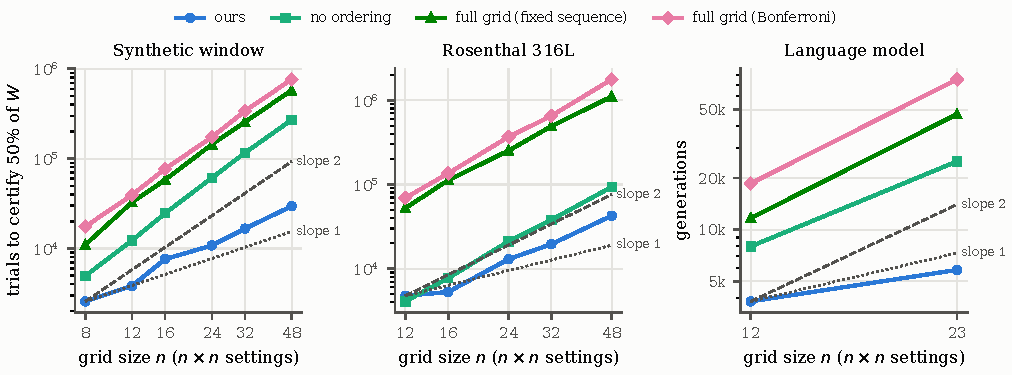
\includegraphics[width=\textwidth]{figs/fig_scaling.pdf}
\caption{Trials to certify half of the safe region as the grid is refined
(fixed budget, log--log). With the ordering the cost grows roughly like
the region's edge (slope 1); without it, and for full grids, like its area
(slope 2).}
\label{fig:scaling}
\end{figure*}

\paragraph{Fixed budget.} Table~\ref{tab:scaling} and
Figure~\ref{fig:scaling}. The gap to the
unordered method grows with resolution (synthetic: 3.2$\times$ at $16^2$,
9.1$\times$ at $48^2$), as the edge-vs-area bounds predict. The full grids
pay for the whole area; fixed-sequence testing helps them by only
20--40\%. At $24\times24$, to certify 70\% of the region, ours needs
5.0$\times$ fewer trials than no ordering on the synthetic window,
1.5--1.7$\times$ on Rosenthal 316L and 1.3$\times$ on the drug screen.

\begin{table}[t]
\centering\small
\caption{Fixed confidence on the synthetic window (good side information;
median of 4 runs). LB: Theorem~\ref{thm:lb}. The target was fully
certified in 23 of 24 runs (the exception, at $32^2$, hit a probe
time-out, a heuristic outside Theorem~\ref{thm:search}).}
\label{tab:fc}
\begin{tabular}{lrrrrr}
\toprule
 & \multicolumn{3}{c}{with the ordering} & \multicolumn{2}{c}{without} \\
grid & search & LB & ratio & per-setting & LB \\
\midrule
$8^2$  & 14.2k & 3.4k & 4.2 & 21.9k & 4.5k \\
$16^2$ & 50.3k & 8.8k & 5.7 & 100.0k & 18.7k \\
$32^2$ & 165.6k & 19.4k & 8.5 & 457.7k & 77.0k \\
$48^2$ & 334.6k & 24.8k & 13.5 & --- & 174.4k \\
\midrule
LM $12^2$ & \TBD{} & \TBD{} & \TBD{} & \TBD{} & \TBD{} \\
\bottomrule
\end{tabular}
\end{table}

\begin{figure}[t]
\centering
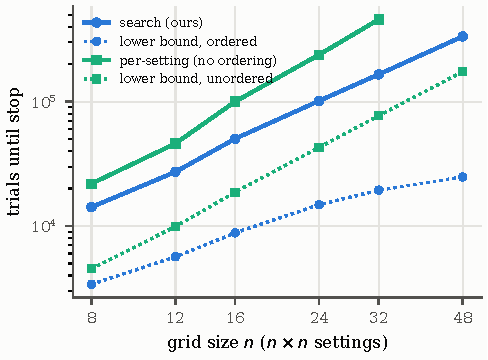
\includegraphics[width=\columnwidth]{figs/fig_fixed_conf.pdf}
\caption{Fixed confidence on the synthetic window: cost at the stopping
time and the lower bounds of Theorem~\ref{thm:lb}.}
\label{fig:fc}
\end{figure}

\paragraph{Fixed confidence.} Table~\ref{tab:fc} and
Figure~\ref{fig:fc}. The ordered bound grows
roughly linearly in $n$ and the unordered one quadratically, as
Theorem~\ref{thm:lb} predicts. Both methods pay a similar multiple-testing
price over their own bound (per-setting: 4.8--5.9$\times$;
$\ln(16MN/(\alpha w))/K_1\approx5$ at $32^2$); the search's extra growth
with $n$ is the $O(\log n)$ probe factor. With optimistic side information
at $32^2$ the search needs 215k trials against 458k without the ordering.

\paragraph{Validity.} With every setting exactly at the tolerance (the
worst case), the false-certification rate is 0--2.75\% across
configurations at $\alpha=5\%$ (400 runs each); no unsafe setting was
certified in any efficiency run.

\paragraph{Model-based baseline.} The GP level-set certificate certifies an
unsafe setting in 40--100\% of runs at confidence parameter 2 and still
7.5--20\% at 4, where it certifies at most 69\% (drug screen) and typically
under 25\% of the region; ours: 0\% and 54--84\%. Language model:
\TBD{}.

\paragraph{Ablations.} The ordering and the allocation rule matter most
(no ordering +69 to +213\%; greedy allocation +63 to +94\%); weights,
pooling and bet seeding give smaller gains; a fixed maximum bet fails when
relevant rates are near the tolerance.

\paragraph{When monotonicity fails.} A pocket of unsafe settings inside the
region is certified by spreading in 75--92\% of runs; an audit re-testing
every certified setting (about 1.2$\times$ the budget) catches gross
violations (96--100\%) but rarely mild ones (4--9\%).

% =====================================================================
\section{Related work}

\emph{Anytime-valid inference and e-values:} \citet{ville1939,
shafer2021, ramdas2023savi, vovk2021evalues, wang2022ebh,
waudbysmith2024betting}. \emph{Multiple testing with structure:} closed
testing \citep{marcus1976closed}, sequential rejection
\citep{goeman2010sequential}, graphical procedures
\citep{bretz2009graphical}, closure for monotone bi-factorial dose designs
\citep{hellmich2005closure}. \emph{Adaptive testing and bandits:}
\citet{jamieson2018bandit, xu2021unified}; thresholding bandits
\citep{locatelli2016tbp} and their monotone versions
\citep{garivier2017dose, cheshire2020shape, cheshire2021problem}; lower
bounds \citep{garivier2016optimal, kaufmann2016complexity,
garivier2019explore}; multi-fidelity best-arm identification
\citep{poiani2022multifidelity, poiani2024optimal}. \emph{Risk control for
configurations and LLM evaluation:} \citet{angelopoulos2025ltt,
laufer2023pareto, quach2024conformal, joshi2025multirisk}; anytime-valid
evaluation of a single system \citep{zhou2026celeus, zhou2026auditing}.
\emph{Predictions and simulators inside tests:} prediction-powered
inference and e-values \citep{angelopoulos2023ppi, csillag2025ppe}, active
inference \citep{zrnic2024active}, simulator-guided betting for one robot's
mean performance \citep{chen2026simtoreal, chen2026certificates}; we use
side information only for allocation and weights, over a whole region.
\emph{Safe exploration and level sets:} \citet{sui2015safeopt,
losalka2023monotone, losalka2024noregret, gotovos2013lse, mason2022lse}.
\emph{Applications:} adaptive experimental design for AM process
parameters \citep{beam2026}; dose finding for combinations
\citep{wages2011pocrm}.

\section{Limitations}

Assumption~A is load-bearing (Section~\ref{sec:exp}); thin regions gain
less at coarse resolution; the multiple-testing factor dominates the gap
to the lower bound; the language-model study uses a small model and
automatic judges; the manufacturing studies are simulated with placeholder
calibrations.

\bibliographystyle{plainnat}
\bibliography{references}

% =====================================================================
\appendix
\onecolumn
\section{Proofs}\label{app:theory}

\subsection{Setup}
Trial $t=1,2,\dots$ is run at $x_t$ and yields $Y_t\in\{0,1\}^M$. Given the
past and $x_t=x$, $Y_t\sim P_x$, independently of the past. Let
$\mathcal F_t=\sigma(x_1,Y_1,\dots,x_t,Y_t,U)$, where $U$ is independent side
information (simulator output, pilot data, internal randomization). The
allocation $x_t$ is $\mathcal F_{t-1}$-measurable: trials in a batch are
chosen before any of them is observed, and processing them one at a time
in a fixed order keeps this property.

\begin{lemma}\label{lem:supermart}
If $p_m(x)\ge\eps_m$ then $K_{m,x}$ is a nonnegative supermartingale with
respect to $(\mathcal F_t)$. If $p_m(x)\le q\eps_m$, the rejection process
$R_{m,x}(t)=\prod_{s\le t:x_s=x}(1+\mu_s(Y_{s,m}-q\eps_m))$,
$\mu_s\in[0,1/(q\eps_m))$ predictable, is a nonnegative supermartingale.
\end{lemma}
\begin{proof}
Nonnegativity: $1+\lambda(\eps-1)\ge 1-c>0$. On $\{x_t=x\}$,
$\E[K(t)\mid\mathcal F_{t-1}] = K(t-1)(1+\lambda_t(\eps-p_m(x)))\le K(t-1)$,
since $\lambda_t$ and $x_t$ are $\mathcal F_{t-1}$-measurable and the
conditional law of $Y_t$ given $\mathcal F_{t-1}$ and $x_t=x$ is $P_x$. On
$\{x_t\ne x\}$, $K(t)=K(t-1)$. The rejection process is identical with the
roles of failures and successes exchanged. A fixed-weight average of such
processes (our hedge) is again a nonnegative supermartingale.
\end{proof}

\subsection{Validity of the cone rule}\label{app:valid}
\begin{proof}[Proof of Theorem~\ref{thm:valid}]
Let $D=\{(m,y):p_m(y)\ge\eps_m\}$. Under Assumption~A, if $(m,x)\in D$ and
$y\preceqm x$ then $p_m(y)\ge p_m(x)\ge\eps_m$, so $\{m\}\times\Cone_m(x)
\subseteq D$. Let $E(t)=\sum_{(m,y)\in D}w_{m,y}K_{m,y}(t)$, a nonnegative
supermartingale by Lemma~\ref{lem:supermart} with $E(0)\le1$. A false
certification of $(m,x)\in D$ at $t$ means $1/\alpha\le S_m(x,t)\le E(t)$.
By Ville's inequality $\P(\sup_tE(t)\ge1/\alpha)\le\alpha$.
\end{proof}
Remarks: nothing about the allocation is used beyond predictability;
certification is sticky, and the bound covers ``ever certified''; with
uniform weights $S_m(x)\ge\max_{y\in\Cone_m(x)}wK_y$, so the cone rule
certifies everything Bonferroni with spreading certifies.

\subsection{Correctness of the search}
\begin{proof}[Proof of Theorem~\ref{thm:search}, correctness]
Validity is Theorem~\ref{thm:valid}. Completeness: let $G$ be the event
that no $(m,x)$ with $p_m(x)\le q\eps_m$ is rejected directly. By
Lemma~\ref{lem:supermart}, Ville and a union bound over $MN$ pairs,
$\P(G^c)\le\beta$. On $G$ no $x\in T$ is rejected or excluded: a spread
rejection of $x$ for $m$ comes from a direct rejection at some $y$ with
$x\preceqm y$, but then $p_m(y)\le p_m(x)\le q\eps_m$, contradicting $G$;
exclusion through another mode is the same argument for that mode.
Termination: every probe ends almost surely (if $p<\eps$ the certification
statistic has positive expected log-growth under the hedge's best fixed
bet; if $p>q\eps$ the rejection process does; since $q<1$ every $p$ is
covered), each probe decides at least one configuration, and $\cX$ is
finite. So on $G$, $\tau<\infty$ and $T\subseteq C$.
\end{proof}

\subsection{Expected passage times}
\begin{lemma}[Wald]\label{lem:wald}
Let $Z_k=\sum_{i\le k}\xi_i$ with $\xi_i$ i.i.d., bounded, $\E\xi=g>0$, and
$\tau=\min\{k:Z_k\ge c\}$. Then $\E\tau\le(c+b)/g$, $b=\operatorname{ess\,sup}\xi$.
\end{lemma}
\begin{proof}
$\E\tau<\infty$ for positive drift with bounded increments; by Wald's
identity $\E Z_\tau=g\E\tau$, and $Z_\tau\le c+b$.
\end{proof}
Applied to the log-wealth of the best fixed bet in the hedge (held with
weight $1/16$) and $S_m(x)\ge w_{m,x}K_{m,x}$: a setting with rate $p<\eps$
sampled exclusively is certified within an expected
$T_c(p)=(\ln(16/(\alpha w))+\ln(1+\lambda^*\eps))/g_c(p)$ trials, where
$g_c(p)=\max_j\E\ln(1+\lambda_j(\eps-Y))$. Likewise rejection at $p>q\eps$
within $T_r(p)=(\ln(5MN/\beta)+b')/g_r(p)$. This gives
Theorem~\ref{thm:oracle} by summing over the cover (plus $B$ per cover
point when certification is checked once per batch).

\begin{proof}[Proof sketch of Theorem~\ref{thm:search}, cost]
Galloping brackets the edge in $\lceil\log_2(d+1)\rceil+1$ probes and
bisection closes the bracket in at most as many; probes elsewhere only
decide configurations earlier. A probe ends at the first of two passage
times, so its expected length is at most $\min(T_c,T_r)\le C^*$. Overshoot
is at most $B$ per probe. Probes for different modes at one configuration
share trials, which only reduces cost.
\end{proof}

\subsection{Lower bounds}
We use the transportation lemma \citep[Lemma~1]{kaufmann2016complexity}: for
instances $\nu,\nu'$, a stopping time $\tau$ and $E\in\mathcal F_\tau$,
$\sum_x\E_\nu[N_x(\tau)]\KL(\nu_x,\nu'_x)\ge\kl(\P_\nu(E),\P_{\nu'}(E))$.
It needs only $\E_\nu[\tau]<\infty$ (otherwise there is nothing to prove):
then $\tau<\infty$ $\nu$-a.s., the restriction of $\P_\nu$ to
$\mathcal F_\tau$ is absolutely continuous with respect to that of
$\P_{\nu'}$ with density the likelihood ratio at $\tau$, Wald's identity
gives the left side as the expected log-likelihood ratio, and the
data-processing inequality gives the right side; $\tau$ may be infinite
under $\nu'$. If $\P_{\nu'}(E)\le\alpha$ the right side is at least
$g(\P_\nu(E))$, and if $\P_{\nu'}(E)\ge1-\beta$ it is at least
$f(\P_\nu(E))$. We restrict to instances with independent modes (a lower
bound on a subclass is a lower bound), so KL adds over modes, and a trial
at $y$ counts once in every constraint that involves $y$.

\begin{proof}[Proof of Theorem~\ref{thm:lb}]
(i) For $m$ and $t$, let $\nu'$ set $p'_m(y)=\max(p_m(y),\eps_m+\eta)$ for
$y\preceqm t$ and leave everything else unchanged. $\nu'$ satisfies
Assumption~A: the riskier cone of $t$ is closed toward risk, and raising a
monotone function to at least a constant on such a set keeps it monotone
(check the three cases of a comparable pair). In $\nu'$, $t$ is unsafe, so
$\P_{\nu'}(T\subseteq C)\le\alpha$, while
$\P_\nu(\tau<\infty,T\subseteq C)\ge1-\beta$; apply the lemma and let
$\eta\to0$.

(ii) Lowering alternative: $p''_m(z)=q\eps_m$, everything else unchanged.
This keeps Assumption~A because every setting strictly safer than $z$ has
$p_m\le q\eps_m$ and every riskier one has $p_m\ge p_m(z)>q\eps_m$. In
$\nu''$, $z\in T$, so $\P_{\nu''}(z\in C)\ge1-\beta$, giving
$A_z\ge f(\pi)$ with $\pi=\P_\nu(z\in C)$. Raising alternative: as in (i)
with $t$ replaced by $z$; $z$ is unsafe there, giving $B_z\ge g(\pi)$ for
the same $\pi$.

$R$ is convex: its lower-left boundary is $B=g(f^{-1}(A))$ on the range
of $f$, an increasing convex function composed with a decreasing convex
one. Replacing $R$ by finitely many supporting half-planes
$wA+(1-w)B\ge\min_\pi[wf(\pi)+(1-w)g(\pi)]$ gives a linear program with a
smaller value, which is what we report.

Without the ordering, alternatives may change a single setting $x$, so the
constraints decouple: for $x\in T$, $n_x\ge K_1/\min_m\KL(p_m(x)\|\eps_m)$;
for safe $x\notin T$, $n_x\ge\min_\pi\max(f(\pi)/R_x, g(\pi)/C_x)$ with
$R_x=\sum_{m:p_m(x)>q\eps_m}\KL(p_m(x)\|q\eps_m)$ and
$C_x=\min_m\KL(p_m(x)\|\eps_m)$; for unsafe $x$,
$n_x\ge\kl(\alpha,1-\beta)/R_x$.
\end{proof}

\paragraph{Points to check.} (1) Lemma~\ref{lem:supermart} with batched
allocation; (2) the closed-testing interpretation of the cone rule;
(3) that no target configuration is rejected by spreading or exclusion on
$G$; (4) the transportation lemma when $\tau$ may be infinite under the
alternative; (5) that the alternatives keep Assumption~A, and the sharing
of trials across modes; (6) convexity of $R$; (7) the probe count with
spreading from other rows.

\end{document}
